\documentclass{article}
\usepackage[utf8]{inputenc}

\usepackage[a4paper, total={6in, 9in}]{geometry}

\title{Mapper \\ \vspace{0.2cm} \large Topological Data Analysis}
\author{Jana Řežábková, Jan Joneš}
\date{15. 1. 2021}

\usepackage{amsmath}
\usepackage{amssymb}
\usepackage{hyperref}
\usepackage{graphicx}
\usepackage{graphbox}
\usepackage{caption}
\usepackage{subcaption}

\graphicspath{{./figures/}}

\begin{document}

\maketitle

\section{Introduction}

Visualization of high-dimensional data is hard.
In the field of topological data analysis, Mapper~\cite{mapper} is one popular method used for data visualization.

In this report we provide a simple yet fast implementation of Mapper in Python that works on 3D points.

We describe the Mapper algorithm in Section~\ref{sec:alg}.
We provide details of our implementation in Section~\ref{sec:impl}.
We report results of running our implementation on several examples in Section~\ref{sec:res}.
Finally, we conclude this report in Section~\ref{sec:concl}.

\section{Algorithm}\label{sec:alg}

Input to the Mapper algorithm is finite point cloud $X \subset \mathbb{R}^3$.
We demonstrate how the algorithm works on an example of torus whose points are shown in Figure~\ref{fig:torus-points}.

\begin{figure}[ht]
    \centering
    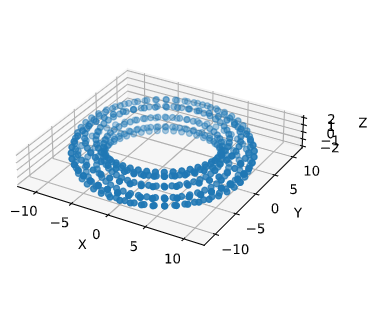
\includegraphics[width=0.7\columnwidth]{torus-point-cloud}
    \caption{Point cloud of torus example.}
    \label{fig:torus-points}
\end{figure}

The algorithm first applies filter function $f: X \to I$ where $I \subseteq \mathbb{R}$, mapping each point to real space.
Filter function can be arbitrary and its choice usually depends on the input data.
Commonly used filter functions are
\begin{itemize}
    \item specific coordinate, e.g., y coordinate $f((x, y, z)) = y$,
    \item distance from point $\mathbf{p}$, i.e., $f(\mathbf{x}) = \lVert \mathbf{x} - \mathbf{p} \rVert_2$, where origin is usually used as $\mathbf{p}$.
\end{itemize}
Applying filter function to our torus example is demonstrated in Figure~\ref{fig:torus-filter}.

\begin{figure}[ht]
    \centering
    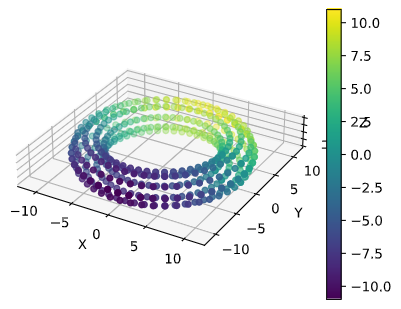
\includegraphics[width=0.4\columnwidth]{torus-y-coor}
    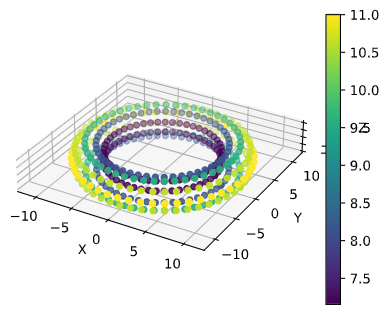
\includegraphics[width=0.4\columnwidth]{torus-distance-from-origin}
    \caption{Different filter functions applied to our torus example.
        Y coordinate is used on the left and distance from origin is used on the right.
        Value of the filter function is illustrated using color range.}
    \label{fig:torus-filter}
\end{figure}

We continue by splitting interval $I$ into overlapping bins.
Formally, we take $\mathcal{U} = \{ U_\alpha \}_{\alpha \in A}$ finite covering of $I$.
Usually, uniform covering is used.
Then, it is enough to specify number of bins and ratio of overlap.
Splitting interval using covering of our torus example is demonstrated in Figure~\ref{fig:torus-cover}.

\begin{figure}[ht]
    \centering
    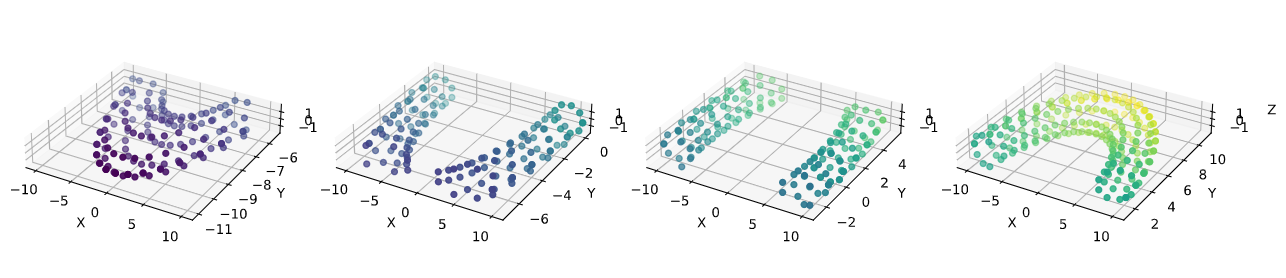
\includegraphics[width=0.9\columnwidth]{torus-partition-4-25}
    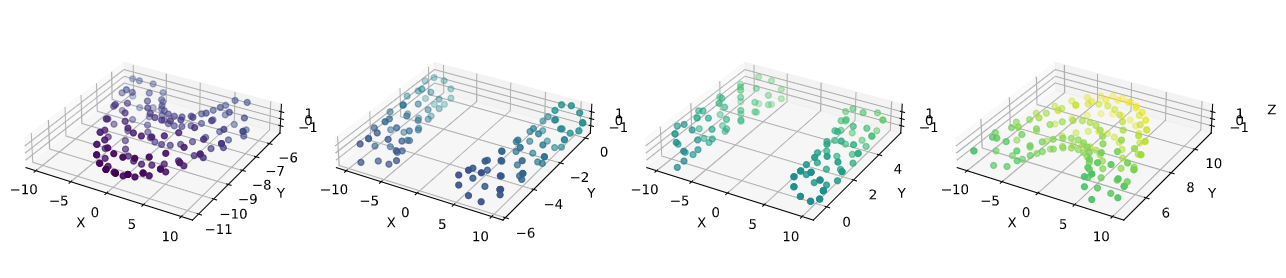
\includegraphics[width=0.9\columnwidth]{torus-partition-4-05}
    \caption{Different coverings applied to our torus example.
        We use 4 bins with 25~\% overlap in the top row and 5~\% overlap in the bottom row.
        We also color vertices by their original filter values.}
    \label{fig:torus-cover}
\end{figure}

We then perform clustering in each interval obtained from covering.
Formally, we cluster points $f^{-1}(U_\alpha)$ for each $\alpha \in A$.
Clustering method can be again arbitrary chosen and its parameters must be tweaked in order to obtain good results in later stages of the algorithm.
Commonly used clustering schemes include agglomerative clustering (where we can choose for example single or average linkage), K-Means clustering and ToMATo~\cite{tomato}.
Clustering our torus example is demonstrated in Figure~\ref{fig:torus-cluster}.

\begin{figure}[ht]
    \centering
    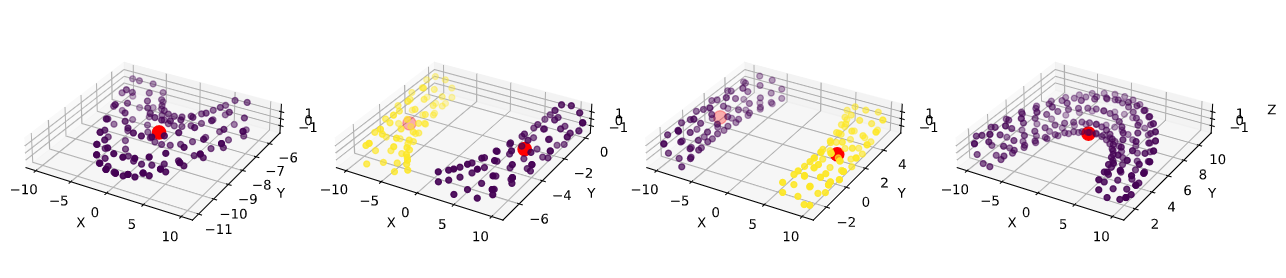
\includegraphics[width=0.9\columnwidth]{torus-clustering}
    \caption{Agglomerative clustering with average linkage applied to our torus example.
        Each cluster's center is represented by bigger red dot.}
    \label{fig:torus-cluster}
\end{figure}

Output of the Mapper algorithm is graph $G$ whose vertices are clusters from all $f^{-1}(U_\alpha)$ and
$$
    (u, v) \in E_G \Leftrightarrow u \cap v \neq \emptyset \mbox{,}
$$
i.e., there is an edge between clusters if there is nonempty intersection between them (which happens thanks to overlaps in $\mathcal{U}$).
Resulting Mapper graph for our torus example is depicted in Figure~\ref{fig:torus-mapper}.

\begin{figure}[ht]
    \centering
    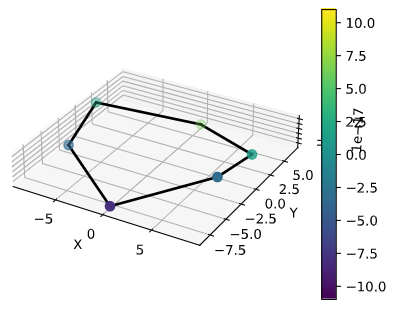
\includegraphics[align=c, width=0.4\columnwidth]{torus-graph-3d}
    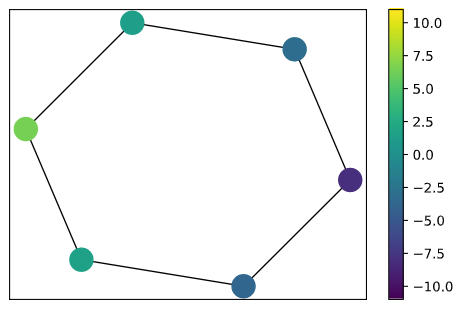
\includegraphics[align=c, width=0.4\columnwidth]{torus-graph-2d}
    \caption{Mapper graph of our torus example.
        The same graph is depicted in space on the left and in plane on the right.
        In space, nodes are positioned at their corresponding cluster centers.
        We also color nodes by their corresponding filter values.}
    \label{fig:torus-mapper}
\end{figure}

Finally, we treat the resulting Mapper graph as simplicial complex and compute its persistent homology.
We need filtration to compute persistent homology and we have two obvious approaches for computing filtration from the Mapper graph:
\begin{enumerate}
    \item Perform Rips filtration on the graph in space.
    \item Start with empty filtration.
          Add vertices to the filtration incrementally for increasing filter values.
          Formally, add vertex $v$ to filtration at $f(v)$.
          Add edge as soon as both of its vertices are added, i.e., add edge $(u, v)$ at $\max\,\{ f(u), f(v) \}$.
\end{enumerate}
Persistence diagrams of both approaches applied to our torus example are shown in Figure~\ref{fig:torus-persistence}.

\begin{figure}[ht]
    \centering
    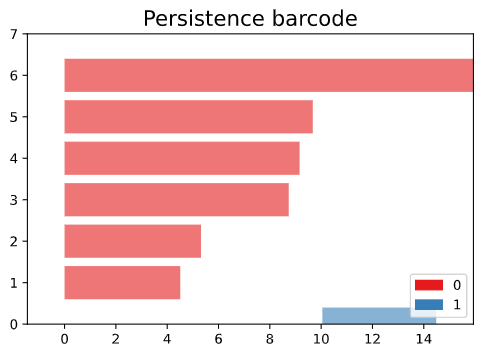
\includegraphics[width=0.4\columnwidth]{torus-rips-barcode}
    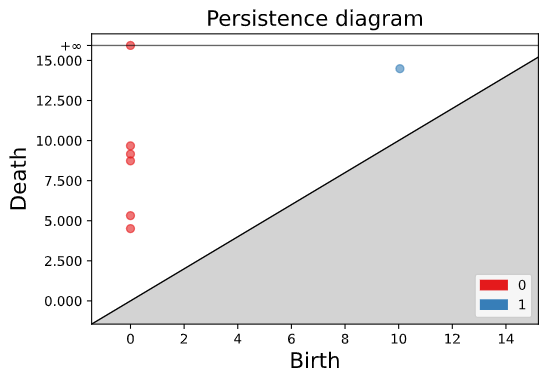
\includegraphics[width=0.4\columnwidth]{torus-rips-persistence-diagram}
    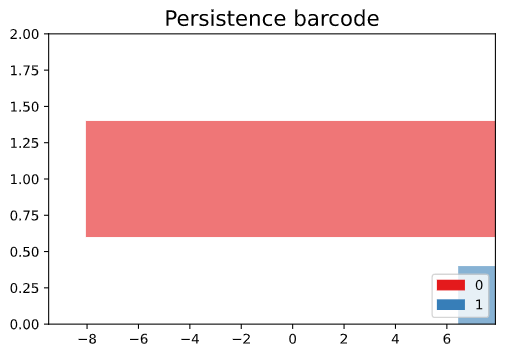
\includegraphics[width=0.4\columnwidth]{torus-barcode}
    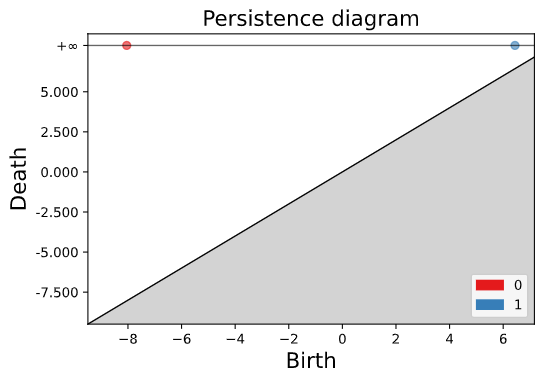
\includegraphics[width=0.4\columnwidth]{torus-persistence-diagram}
    \caption{Persistence barcodes and diagrams of our torus example computed using Rips filtration (in the top row) and filter-function-based filtration (in the bottom row).}
    \label{fig:torus-persistence}
\end{figure}

\section{Implementation}\label{sec:impl}

We implement the Mapper algorithm as a Python library.
It contains all steps of the algorithm described in Section~\ref{sec:alg} and also code necessary to plot the corresponding figures and diagrams.
We also include Python scripts for running our implementation on examples presented in Section~\ref{sec:res} and a few more.

We implement most of the algorithm ourselves, using NumPy~\cite{numpy} for computations and Matplotlib~\cite{matplotlib} and Networkx~\cite{networkx} for plotting.
However, we use Gudhi~\cite{gudhi} implementation of ToMATo clustering and persistent homology computation and scikit-learn~\cite{scikit} implementation of other clustering schemes.

Our implementation includes basic filter functions (chosen coordinate, distance from point), uniform cover (with number of bins and overlap parameters) and aforementioned clustering schemes (proxy for other libraries).
Thanks to flexible modular architecture, more filter functions, cover methods and clustering schemes can be implemented and incorporated into our Mapper library easily.

All code is available online at \url{https://github.com/janarez/mapper}.
The repository contains documentation including instructions for using the library and running examples.

\section{Results}\label{sec:res}

We run our Mapper algorithm on a point cloud of human hand consisting of almost 13 thousand vertices (Figure~\ref{fig:hand-points}).
We use y coordinate filter function, five bins with 25~\% overlap and ToMATo clustering (Figure~\ref{fig:hand-cluster}).
The hand is clearly visible in the resulting graph and its five fingers are well separated with the thumb starting earlier than the other four fingers (Figures~\ref{fig:hand-space} and~\ref{fig:hand-plane}).

\begin{figure}[ht]
    \centering
    \begin{subfigure}[c]{0.3\columnwidth}
        \centering
        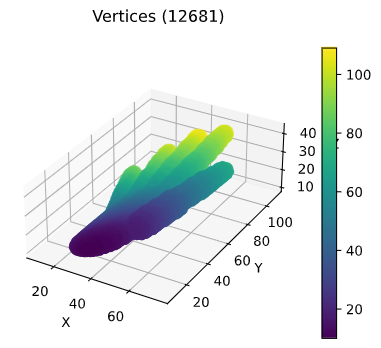
\includegraphics[width=\textwidth]{hand-point-cloud}
        \caption{Point cloud}
        \label{fig:hand-points}
    \end{subfigure}
    \begin{subfigure}[c]{0.3\columnwidth}
        \centering
        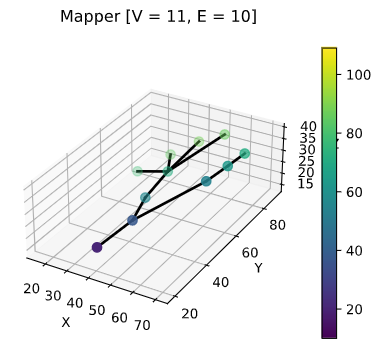
\includegraphics[width=\textwidth]{hand-graph-3d}
        \caption{Graph in space}
        \label{fig:hand-space}
    \end{subfigure}
    \begin{subfigure}[c]{0.3\columnwidth}
        \centering
        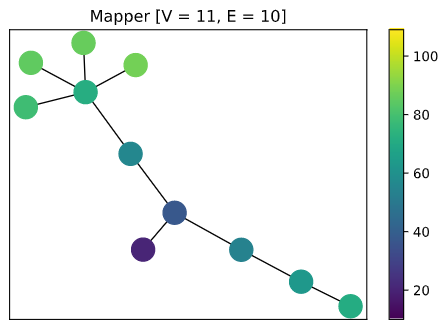
\includegraphics[width=\textwidth]{hand-graph-2d}
        \caption{Graph in plane}
        \label{fig:hand-plane}
    \end{subfigure}
    \begin{subfigure}[c]{0.9\columnwidth}
        \centering
        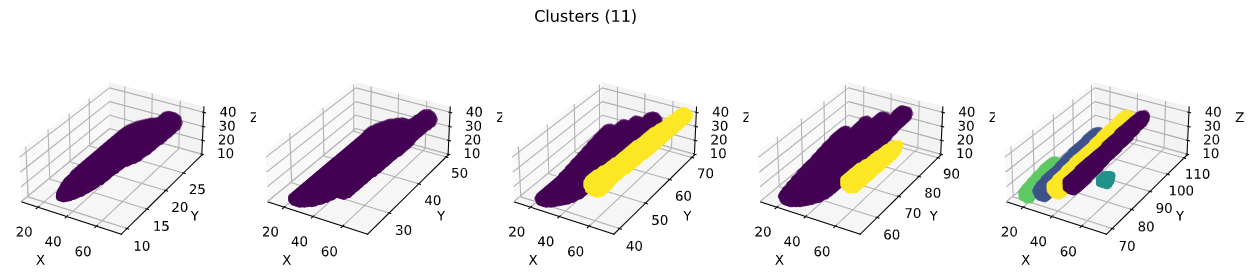
\includegraphics[width=\textwidth]{hand-clusters}
        \caption{Clustering}
        \label{fig:hand-cluster}
    \end{subfigure}
    \caption{Results of running our Mapper algorithm on a point cloud of hand.}
    \label{fig:hand}
\end{figure}

\section{Conclusion}\label{sec:concl}

\bibliographystyle{IEEEtran}
\bibliography{bibliography}

\end{document}
